%%
%% Copyright 2007, 2008, 2009 Elsevier Ltd
%%
%% This file is part of the 'Elsarticle Bundle'.
%% ---------------------------------------------
%%
%% It may be distributed under the conditions of the LaTeX Project Public
%% License, either version 1.2 of this license or (at your option) any
%% later version.  The latest version of this license is in
%%    http://www.latex-project.org/lppl.txt
%% and version 1.2 or later is part of all distributions of LaTeX
%% version 1999/12/01 or later.
%%
%% The list of all files belonging to the 'Elsarticle Bundle' is
%% given in the file `manifest.txt'.
%%

%% Template article for Elsevier's document class `elsarticle'
%% with numbered style bibliographic references
%% SP 2008/03/01

\documentclass[preprint,12pt, a4paper]{elsarticle}

%% Use the option review to obtain double line spacing
%% \documentclass[authoryear,preprint,review,12pt]{elsarticle}

%% For including figures, graphicx.sty has been loaded in
%% elsarticle.cls. If you prefer to use the old commands
%% please give \usepackage{epsfig}

%% The amssymb package provides various useful mathematical symbols
\usepackage{amssymb}
\usepackage{hyperref}
\setlength{\parindent}{0pt}
%% The amsthm package provides extended theorem environments
%% \usepackage{amsthm}

%% The lineno packages adds line numbers. Start line numbering with
%% \begin{linenumbers}, end it with \end{linenumbers}. Or switch it on
%% for the whole article with \linenumbers.
%\usepackage{lineno}

\usepackage{pgfplots}

\usepackage[polish]{babel}
\usepackage[T1]{fontenc}
\usepackage{graphicx}
\graphicspath{ {./fig/} }

\usetikzlibrary{arrows.meta}
\tikzstyle{oneArrowStyle} = [-Stealth,line width = 1]
\tikzstyle{oneArrowinverseStyle} = [Stealth-,line width = 1]

\newcommand{\SoftwareName}{GTest }

\journal{SoftwareX}

\begin{document}
\renewcommand{\labelenumii}{\arabic{enumi}.\arabic{enumii}}

\begin{frontmatter}
%--- INSTRUCTIONS TO BE DELETED OR COMMENTED BEFORE SUBMISSION

  {\large\textbf{SoftwareX article template Version 4 (November 2023)}}
  Before you complete this template, a few important points to note:
  \begin{itemize}
\item	This template is for an original SoftwareX article. If you are submitting an update to a software article that has already been published, please use the Software Update Template found on the Guide for Authors page.
\item	The format of a software article is very different to a traditional research article. To help you write yours, we have created this template. We will only consider software articles submitted using this template.
\item	It is mandatory to publicly share the code/software referred to in your software article. You’ll find information on our software sharing criteria in the SoftwareX \href{https://www.elsevier.com/journals/softwarex/2352-7110/guide-for-authors}{Guide for Authors}.
\item	It’s important to consult the \href{https://www.elsevier.com/journals/softwarex/2352-7110/guide-for-authors}{Guide for Authors} when preparing your manuscript; it highlights mandatory requirements and is packed with useful advice.
\end{itemize}
%
Still got questions?
Email our editorial team at softwarex@elsevier.com.

\textbf{Now you are ready to fill in the template below. As you complete each section, please carefully read the associated instructions. All sections are mandatory, unless marked optional.
Once you have completed the template, delete these instructions. In addition, please delete the instructions in the template (the text written in italics).}
%--- END OF INSTRUCTIONS TO BE DELETED OR COMMENTED BEFORE SUBMISSION

%% Title, authors and addresses

%% use the tnoteref command within \title for footnotes;
%% use the tnotetext command for theassociated footnote;
%% use the fnref command within \author or \address for footnotes;
%% use the fntext command for theassociated footnote;
%% use the corref command within \author for corresponding author footnotes;
%% use the cortext command for theassociated footnote;
%% use the ead command for the email address,
%% and the form \ead[url] for the home page:
%% \title{Title\tnoteref{label1}}
%% \tnotetext[label1]{}
%% \author{Name\corref{cor1}\fnref{label2}}
%% \ead{email address}
%% \ead[url]{home page}
%% \fntext[label2]{}
%% \cortext[cor1]{}
%% \address{Address\fnref{label3}}
%% \fntext[label3]{}

\title{Title (Name of your software: Then a short title)}

%% use optional labels to link authors explicitly to addresses:
%% \author[label1,label2]{}
%% \address[label1]{}
%% \address[label2]{}

\author[label1]{A. Author1}
\author[label2]{A. Author2}
\address[label1]{Author1's affiliation, address, email}
\address[label2]{Author2's affiliation, address, email}

\begin{abstract}
%% Text of abstract
\textit{Ca. 100 words. The abstract is followed by a maximum of six keywords
and some mandatory and optional metadata.}

\textit{Your main body of text (sections 1-5 below) should be a maximum 6 pages in total (excluding metadata, tables, figures, references) with a 3000-word limit (we ask that more priority is placed on the word limit versus the page count). Though we strictly insist on the author following the template, in exceptional circumstances, we can be flexible with the page numbers and word limit. In such cases, it should be discussed with the managing editor or publisher prior to submission. All queries regarding the same can be reached at softwarex@elsevier.com.}
\end{abstract}

\begin{keyword}
%% keywords here, in the form: keyword \sep keyword
keyword 1 \sep keyword 2 \sep keyword 3

%% PACS codes here, in the form: \PACS code \sep code

%% MSC codes here, in the form: \MSC code \sep code
%% or \MSC[2008] code \sep code (2000 is the default)

\end{keyword}

\end{frontmatter}

%\linenumbers

\section*{Metadata}
\label{}
\textit{The ancillary data table~\ref{codeMetadata} is required for the sub-version of the codebase. Please replace the italicized text in the right column with the correct information about your current code and leave the left column untouched.}

\begin{table}[!h]
\begin{tabular}{|l|p{6.5cm}|p{6.5cm}|}
\hline
\textbf{Nr.} & \textbf{Code metadata description} & \textbf{Please fill in this column} \\
\hline
C1 & Current code version & For example v42 \\
\hline
C2 & Permanent link to code/repository used for this code version & For example: \url{https://github.com/mozart/mozart2} \\
\hline
C3  & Permanent link to Reproducible Capsule & For example: \url{https://codeocean.com/capsule/0270963/tree/v1}\\
\hline
C4 & Legal Code License   & All software and code must be released under one of the pre-approved licenses listed in the \href{https://www.elsevier.com/journals/softwarex/2352-7110/guide-for-authors}{Guide for Authors}, such as Apache License, GNU General Public License (GPL) or MIT License. Write the name of the license you’ve chosen here. \\
\hline
C5 & Code versioning system used & For example: svn, git, mercurial,
                                   etc. (put none if none is used) \\
\hline
C6 & Software code languages, tools, and services used & For example: C++, python, r, MPI, OpenCL, etc. \\
\hline
C7 & Compilation requirements, operating environments \& dependencies & \\
\hline
C8 & If available Link to developer documentation/manual & For example: \url{http://mozart.github.io/documentation/} \\
\hline
C9 & Support email for questions & \\
\hline
\end{tabular}
\caption{Code metadata (mandatory)}
\label{codeMetadata}
\end{table}

\textit{Optionally, you can provide information about the current executable
software version filling in the left column of
Table~\ref{executabelMetadata}. Please leave the first column as it is.}

\begin{table}[!h]
\begin{tabular}{|l|p{6.5cm}|p{6.5cm}|}
\hline
\textbf{Nr.} & \textbf{(Executable) software metadata description} & \textbf{Please fill in this column} \\
\hline
S1 & Current software version & For example 1.1, 2.4 etc. \\
\hline
S2 & Permanent link to executables of this version  & For example: \url{https://github.com/combogenomics/DuctApe/releases/tag/DuctApe-0.16.4} \\
\hline
S3  & Permanent link to Reproducible Capsule & \\
\hline
S4 & Legal Software License & List one of the approved licenses \\
\hline
S5 & Computing platforms/Operating Systems & For example Android, BSD, iOS, Linux, OS X, Microsoft Windows, Unix-like , IBM z/OS, distributed/web based etc. \\
\hline
S6 & Installation requirements \& dependencies & \\
\hline
S7 & If available, link to user manual - if formally published include a reference to the publication in the reference list & For example: \url{http://mozart.github.io/documentation/} \\
\hline
S8 & Support email for questions & \\
\hline
\end{tabular}
\caption{Software metadata (optional)}
\label{executabelMetadata}
\end{table}


\section{Motivation and significance}
\textit{In this section, we want you to introduce the scientific background and the motivation for developing the software.}

\begin{itemize}
    \item \textit{Explain why the software is important and describe the exact (scientific) problem(s) it solves.}
    \item \textit{Indicate in what way the software has contributed (or will contribute in the future) to the process of scientific discovery; if available, please cite a research paper using the software.}
    \item \textit{Provide a description of the experimental setting. (How does the user use the software?)}
    \item \textit{Introduce related work in literature (cite or list algorithms used, other software etc.).}
\end{itemize}



\section{Software description}

\textit{Describe the software. Provide enough detail to help the reader understand its impact. }

\subsection{Software architecture}

Oprogramowanie \SoftwareName wykorzystuje platformę programistyczną Matlab/Octave oraz silnik gier Unity. Część przeznaczona  dla silnika gier jest napisana w języku C\verb|#|. Implementuje mechanikę rozgrywki w grę typu tower defense. Rolę gracza pełni oprogramowanie napisane w języku Matlab. Komunikacja między oprogramowaniem w Matlab-ie a grą odbywa się na zasadzie kilent-serwer  (fig.~\ref{Fig:architecture}). Gra oczekuje na polecenia nasłuchując na wybranym porcie. Możliwa jest komunikacja zdalna poprzez internet. Oprogramowanie w Matlab-ie  jest zbiorem funkcji pozwalających na realizację badań metod decyzyjnych. Umożliwia pobieranie od gry aktualnych informacje o jej stanie i pozwala na  przekazywanie jej komend sterujących realizujących akcje stawianie nowych wież na planszy oraz wypuszczania nowych przeciwników. 

\begin{figure}
\begin{tikzpicture}
\node[rectangle,draw,minimum width = 3.5cm,minimum height = 1.5cm,label=above:{Player}] (r) at (-2.5,4.5) {Matlab/Octave};
\node[anchor=center,inner sep=0,label=above:{Game}] (game) at (4,4.5) {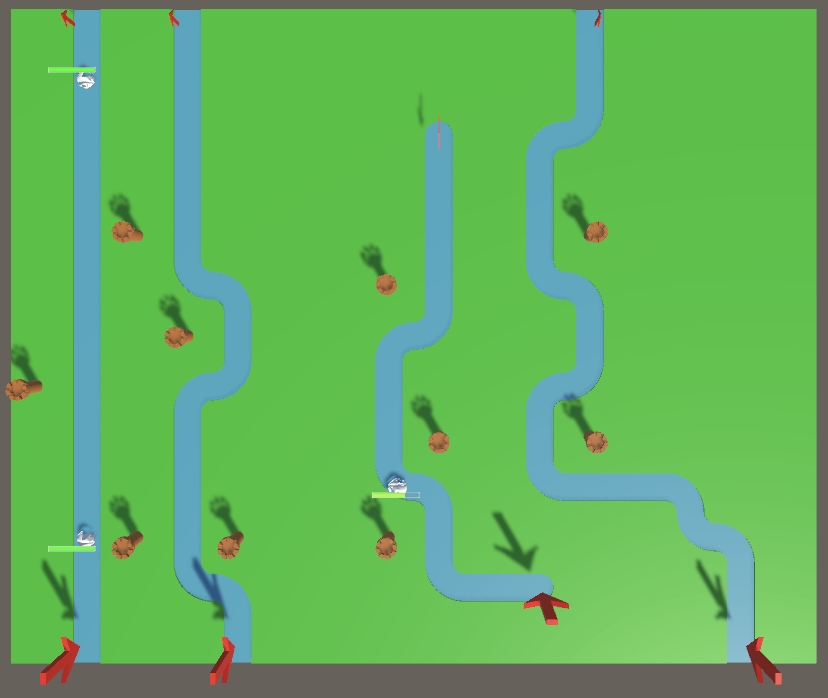
\includegraphics[width=3cm]{images/game.png}} ;
\node[anchor=center,inner sep=0, label=below:{Reports}] (tabaular) at (-2.5,1) {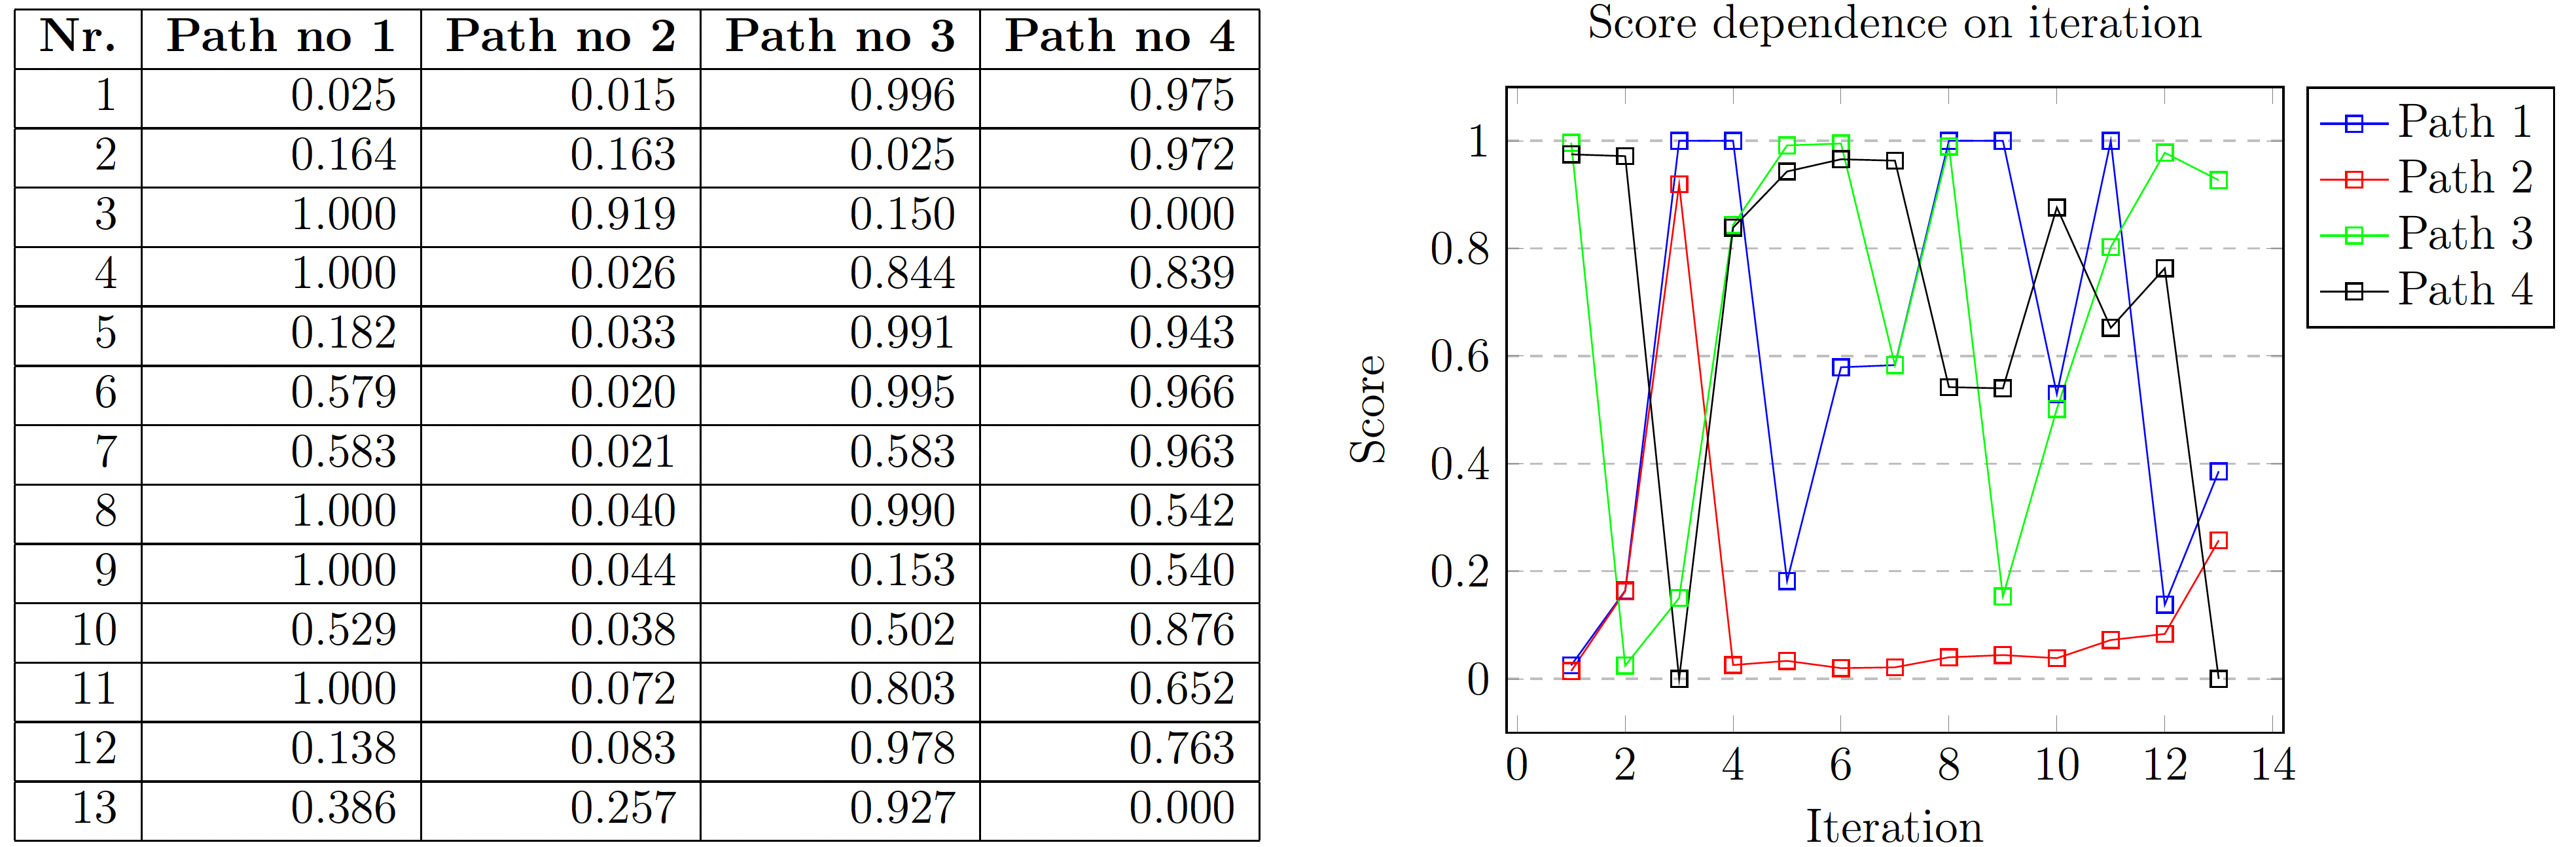
\includegraphics[height=2.5cm]{images/latexReports.png}};
\draw[oneArrowinverseStyle] (r.east) + (0,-0.1) -- ++(3.3,-0.1) node[midway,below]{Answer};
\draw[oneArrowStyle] (r.east) + (0,0.1) -- ++(3.3,0.1) node[midway,above]{Command};
\draw[oneArrowStyle] (r) -- (tabaular);

\end{tikzpicture}

\caption{Architektura systemu}
\label{Fig:architecture}
\end{figure}

Rysunek~\ref{Fig:softwareArchitecture} przedstawia ważniejsze klasy gry tower defense. Jedną z najważniejszych jej klas jest UnityServer realizująca wymianę informacji w formacie XML z oprogramowaniem działającym na platformie programistycznej Matlab. Instancja tej klasy dekoduje otrzymane rozkazy i w zależności od potrzeb komunikuje się z innymi obiektami przekazując im zadania i zbierając potrzebne dane. Klasa ManagementTilemap zajmuje się zarządzaniem najmniejszymi elementami mapy -- tile. Instancja klasy ManagementTilemap zleca instancji klasy CreateTilemap wykonanie tilemap w oparciu o dostępne tile. Gromadzi informacje statystyczne związane z wydarzeniami na kafelkach takich jak przejście  przeciwnika, zabicie przeciwnika itp. Przechowuje informacje o różnych typach tile, a w tym o ich wyglądzie (ma dostęp do ich modeli 3D). Zleca instancji klasy ManagementCost wyznaczenie optymalnej trasy ruchu minimalizującej koszt przejścia od punktu startowego do końcowego. Instancja klasy Towers przechowuje informacje o wieży, jej parametrach oraz wyglądzie. Podobnie instancja klasy EnemyInfo przechowuje informacje o przeciwniku, jego parametrach oraz wyglądzie. Instancja klasy ManagementCash zajmuje się zarządzaniem cash. Wyznacza ile cash mają wieże, ile przeciwnicy i jest odpowiedzialna za prezentowanie tej informacji na HUD-ie i jej aktualizację.  

\begin{figure}
\begin{tikzpicture}
\begin{class}{ManagementTilemap}{-8,20.5}
\end{class}
\begin{class}{CreateTilemap}{-2,20.5}
\end{class}
\begin{class}{UnityServer}{-5,17}
\end{class}
\begin{class}{ManagementCash}{0,13.5}
\end{class}
\begin{class}{Towers}{0,18.4}
\end{class}
\begin{class}{EnemyInfo}{(-1,9}
\end{class}
\begin{class}{ManagementCost}{(-7,6}
\end{class}

\unidirectionalAssociation{ManagementTilemap}{}{}{CreateTilemap}{}{}
\unidirectionalAssociation{ManagementTilemap}{}{}{ManagementCost}{}{}
\unidirectionalAssociation{UnityServer}{}{}{ManagementCost}{}{}
\unidirectionalAssociation{UnityServer}{}{}{ManagementCash}{}{}
\unidirectionalAssociation{UnityServer}{}{}{EnemyInfo}{}{}
\unidirectionalAssociation{UnityServer}{}{}{ManagementTilemap}{}{}
\unidirectionalAssociation{UnityServer}{}{}{Towers}{}{}
\unidirectionalAssociation{Towers}{}{}{CreateTilemap}{}{}
\unidirectionalAssociation{Towers}{}{}{ManagementCash}{}{}
\unidirectionalAssociation{EnemyInfo}{}{}{ManagementCash}{}{}

\node[anchor=center,inner sep=0,label=below:{Tower}] (towerCharacter) at (-10,9) {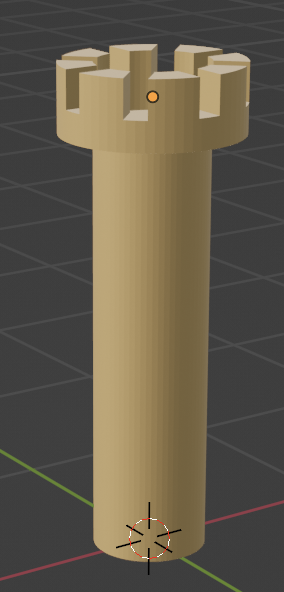
\includegraphics[height=2.5cm]{images/towerCharacter.png}};
\node[anchor=center,inner sep=0,label=below:{Enemy}] (enemyCharacter) at (-10,15.5) {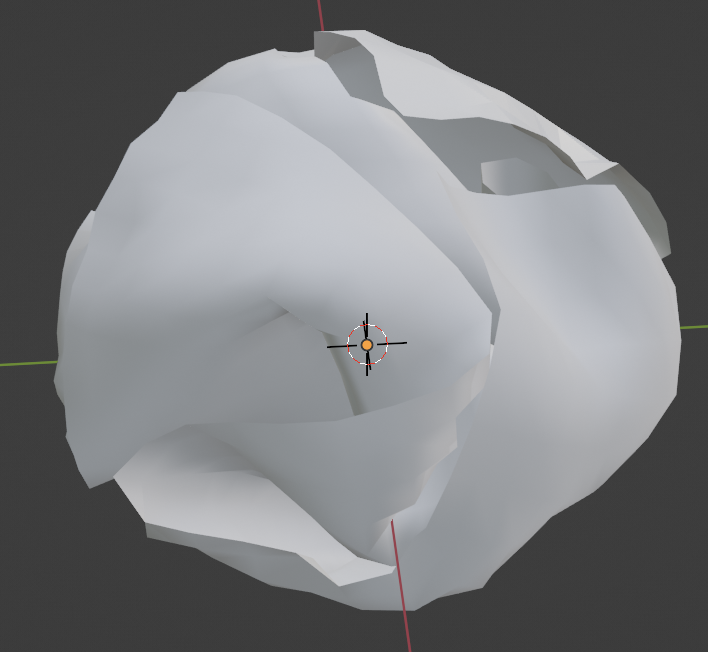
\includegraphics[height=2cm]{images/enemyCharacter.png}};
\node[anchor=center,inner sep=0,label=below:{Tile}] (tileCharacter1) at (-10,18) {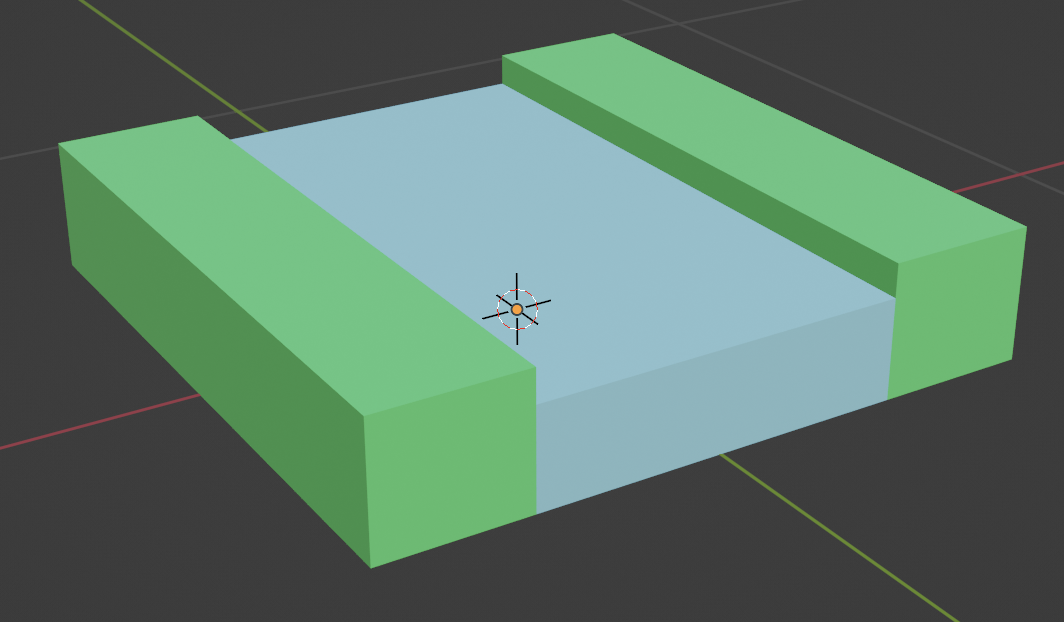
\includegraphics[height=1.5cm]{images/tileCharacter1.png}};
\node[anchor=center,inner sep=0,label=below:{HUD}] (HUD) at (-10,12.5) {
\includegraphics[height=1cm]{images/HUD.png}};

\draw[oneArrowStyle] (UnityServer) -- (towerCharacter);
\draw[oneArrowStyle] (UnityServer) -- (enemyCharacter);
\draw[oneArrowStyle] (ManagementCost) -- (towerCharacter);
\draw[oneArrowStyle] (EnemyInfo) -- (enemyCharacter);
\draw[oneArrowStyle] (Towers) -- (towerCharacter);
\draw[oneArrowStyle] (ManagementCash) -- (HUD);
\draw[oneArrowStyle] (ManagementTilemap) -- (tileCharacter1);


\end{tikzpicture}

\caption{Software architecture: uproszczony diagram klas z dodanymi obiektami 3D powiązanymi z klasami}
\label{Fig:softwareArchitecture}
\end{figure}



\textit{  Give a short overview of the overall software architecture; provide a pictorial overview where possible; for example, an image showing the components. If necessary, provide implementation details.}

 \subsection{Software functionalities}
\textit{  Present the major functionalities of the software.}

 \subsection{Sample code snippets analysis (optional)}


\section{Illustrative examples}

\textit{Provide at least one illustrative example to demonstrate the major
functions of your software/code.}

\textit{\textbf{Optional}: you may include one explanatory  video or screencast that will appear next to your article, in the right hand side panel. Please upload any video as a single supplementary file with your article. Only one MP4 formatted, with 150MB maximum size, video is possible per article. Recommended video dimensions are 640 x 480 at a maximum of 30 frames / second. Prior to submission please test and validate your .mp4 file at  \url{http://elsevier-apps.sciverse.com/GadgetVideoPodcastPlayerWeb/verification} . This tool will display your video exactly in the same way as it will appear on ScienceDirect. }

\begin{table}[!h]
\begin{tabular}{|r|r|r|r|r|}
  \hline
  \textbf{Nr.}&  \textbf{Path no 1}&  \textbf{Path no 2}&  \textbf{Path no 3}&  \textbf{Path no 4}\\
  \hline
  1& -0.518& -0.550& 0.567& 0.501\\
  \hline
  2& -0.228& -0.259& -0.377& 0.864\\
  \hline
  3& 0.454& 0.420& -0.069& -0.805\\
  \hline
  4& 0.103& -0.434& 0.373& -0.043\\
  \hline
  5& -0.445& -0.160& 0.434& 0.171\\
  \hline
  6& -0.105& -0.226& 0.239& 0.093\\
  \hline
  7& 0.136& -0.222& -0.102& 0.188\\
  \hline
  8& 0.446& -0.122& -0.009& -0.316\\
  \hline
  9& 0.367& 0.149& -0.377& -0.139\\
  \hline
  10& 0.083& -0.012& -0.035& -0.037\\
  \hline
  11& 0.184& -0.042& 0.102& -0.244\\
  \hline
  12& -0.381& 0.166& 0.365& -0.149\\
  \hline
  13& -0.318& 0.319& 0.165& -0.166\\
  \hline
\end{tabular}

\caption{Test}
\label{test}
\end{table}

\section{Impact}
\textit{This is the main section of the article and reviewers will weight it appropriately.
Please indicate:}
\begin{itemize}
    \item \textit{Any new research questions that can be pursued as a result of your software.}
    \item \textit{In what way, and to what extent, your software improves the pursuit of existing research questions.}
    \item \textit{Any ways in which your software has changed the daily practice of its users.}
    \item \textit{How widespread the use of the software is within and outside the intended user group (downloads, number of users if your software is a service, citable publications, etc.).}
    \item \textit{How the software is being used in commercial settings and/or how it has led to the creation of spin-off companies.}
    \end{itemize}
\textit{Please note that points 1 and 2 are best demonstrated by
  references to citable publications.}



\section{Conclusions}



\section*{Acknowledgements}
\label{}
\textit{Optional. You can use this section to acknowledge colleagues who don’t qualify as a co-author but helped you in some way. }


%% The Appendices part is started with the command \appendix;
%% appendix sections are then done as normal sections
%% \appendix

%% \section{}
%% \label{}

%% References:
%% If you have bibdatabase file and want bibtex to generate the
%% bibitems, please use
%%
%%  \bibliographystyle{elsarticle-num}
%%  \bibliography{<your bibdatabase>}

%% else use the following coding to input the bibitems directly in the
%% TeX file.

\begin{thebibliography}{00}

%% \bibitem{label}
%% Text of bibliographic item

\bibitem{} Use this style of ordering. References in-text should also use a similar style.

\end{thebibliography}

\textit{If the software repository you used supplied a DOI or another
Persistent IDentifier (PID), please add a reference for your software
here. For more guidance on software citation, please see our guide for
authors or \href{https://f1000research.com/articles/9-1257/v2}{this
  article on the essentials of software citation by FORCE 11}, of
which Elsevier is a member.}

\large{\textbf{Reminder: Before you submit, please delete all
the instructions in this document,
including this paragraph.
Thank you!}}




\end{document}
\endinput
%%
%% End of file `SoftwareX_article_template.tex'.

%%% Local Variables:
%%% mode: latex
%%% TeX-master: t
%%% End:
